
\section{\trFloerEquation{}的解是“\trSomewhereInjective”的}
\label{sec:somewhere-injective}

\subsection{“在 $s$ 上”的\trInjective{}性}
\label{subsec:injectivity-in-s}

我们现在来证明\cref{thm:critical-points-discrete}以及一个\trContinuationPrinciple——后者曾在我们证明\cref{thm:transversality-property}的过程中用到（即下文的\cref{thm:continuation-principle}）。令 $z=s+it$，并设 $u$ 是方程
\[
\frac{\partial u}{\partial s}+J(t,u)\Bigl(\frac{\partial u}{\partial t}-X(t,u)\Bigr)=0
\]
的一个解。这里 $X$ 是 $\RR^{2n}$ 上的一个\trVectorField（它\trPeriodic{}地依赖于时间），并且我们假定 $X$ 与 $J$ 都是 $\cC^\infty$ 类的。凡 $W^{1,p}$ 类（其中 $p>2$）的解 $u$ 事实上都是 $\cC^\infty$ 类的。我们先把这一方程化成 $\RR^2$ 上的一个\trCauchyRiemann{}方程。

\begin{proposition}\label{thm:floer-via-cauchy-riemann}
设 $u$ 是方程
\[
\frac{\partial u}{\partial s}+J(t,u)\Bigl(\frac{\partial u}{\partial t}-X(t,u)\Bigr)=0\text{，}
\]
的一个解。则存在 $W$ 上的一个\trAlmostComplex{}结构 $J$ 与一个\trDiffeomorphism{} $\varphi$，以及一个 $\cC^\infty$ 类的映射 $v\colon\RR^2\to W$，使得
\[
\left\{\begin{array}{l}
\dfrac{\partial v}{\partial s}+J\dfrac{\partial v}{\partial t}=0\\
v(s,t+1)=\varphi(v(s,t))\text{，}
\end{array}\right.
\]
并且对 $(s,t)\in\RR\times[0,1[$，有 $C(u)=C(v)$（$u$ 与 $v$ 有相同的\trCriticalPoint）以及 $R(u)=R(v)$。
\end{proposition}

\begin{proof}
由于 $W\times S^1$ 是\trCompact{}的，$X_t$ 的“流”$\psi_t$ 在整个 $W$ 上有定义，于是我们有一个映射
\[
\psi_t\colon W\longrightarrow W
\qquad\text{满足 }\frac{d}{dt}\psi_t=X_t\circ\psi_t\ \text{且}\ \psi_0=\mathrm{Id}\text{，}
\]
令 $v(s,t)=\psi_t^{-1}(u(s,t))$；则
\[
\frac{\partial u}{\partial s}=(d\psi_t)\Bigl(\frac{\partial v}{\partial s}\Bigr)
\qquad\text{与}\qquad
\frac{\partial u}{\partial t}=(d\psi_t)\Bigl(\frac{\partial v}{\partial t}\Bigr)+X_t(u)\text{，}
\]
从而\footnote{译注：原书此式第二行第二个括号印作 $\frac{\partial v}{\partial s}$；按上行代入 $\frac{\partial u}{\partial t}=(d\psi_t)\bigl(\frac{\partial v}{\partial t}\bigr)+X_t(u)$，第二个括号应为 $\frac{\partial v}{\partial t}$，疑系排印之误，此处径改。——译者注}
\[
\begin{aligned}
0&=\frac{\partial u}{\partial s}+J\Bigl(\frac{\partial u}{\partial t}-X_t(u)\Bigr)\\
&=(d\psi_t)\Bigl(\frac{\partial v}{\partial s}\Bigr)+J(u)(d\psi_t)\Bigl(\frac{\partial v}{\partial t}\Bigr)\\
&=(d\psi_t)\Bigl(\frac{\partial v}{\partial s}+(d\psi_t)^{-1}J(u)(d\psi_t)\Bigl(\frac{\partial v}{\partial t}\Bigr)\Bigr)\text{。}
\end{aligned}
\]
令 $(d\psi_t)^{-1}J(u)(d\psi_t)=\psi_t^\star J(v)$，我们看到 $v$ 是
\[
\frac{\partial v}{\partial s}+\psi_t^\star J(v)\frac{\partial v}{\partial t}=0
\]
的一个解。最后取 $\varphi=\psi_1^{-1}$\footnote{译注：原书此处印作“取 $\varphi=\psi_1$”；由 $v(s,t)=\psi_t^{-1}(u(s,t))$ 与 $u$ 关于 $t$ 的\trPeriodic{}性（$u(s,t+1)=u(s,t)$），并注意 $\psi_{t+1}=\psi_t\circ\psi_1$（由 $X$ 对 $t$ \trPeriodic{}及流的唯一性），即得 $v(s,t+1)=\psi_{t+1}^{-1}(u(s,t+1))=\psi_1^{-1}\bigl(\psi_t^{-1}(u(s,t))\bigr)=\psi_1^{-1}(v(s,t))$，故 $\varphi$ 应取 $\psi_1$ 之逆，此处径改。——译者注}（并把所得的\trComplexStructure{}改名为 $J$；这个改名后的\trComplexStructure{}一般仍依赖于 $t$）便告完成。$\varphi$ 与 $v$ 的诸性质的验证是直接的。
\end{proof}

现在我们把这个命题用起来：证明\cref{thm:critical-points-discrete}（关于\trCriticalPoint{}的定理）等价于证明下面两条陈述所表述的结果。第一条断言，$v$ 的\trCriticalPoint{}所成之集（从而还有 $u$ 的）是离散的。

\begin{lemma}\label{thm:dv-isolated-zeros}
存在一个常数 $\delta>0$，使得 $(dv)_z\neq 0$ 对 $0<|z|<\delta$ 成立。
\end{lemma}

这个引理的证明要用到\textbf{\trSimilarityPrinciple}（similarity principle）（\cref{thm:similarity-principle}），我们把它推迟到后文再行给出。

在陈述第二个结果之前，我们考虑一个具有\cref{thm:floer-via-cauchy-riemann}所给的诸性质的 $\cC^\infty$ 类解 $v\colon\RR^2\to W$。回忆
\[
R(v)=\left\{(s,t)\in\RR^2 \;\Bigm|\;
\begin{array}{l}
\dfrac{\partial v}{\partial s}(s,t)\neq 0,\\[2pt]
v(s,t)\neq x^\pm(t)\ \text{且}\ v(s,t)\notin v(\RR-\{s\},t)
\end{array}\right\}\text{。}
\]

\textbf{定义。}

我们设 $v(\pm\infty,t)=x^\pm(t)$。设 $(s,t)\in\RR^2$。我们把一点 $(s',t)$（$t$ 相同！）称为 $(s,t)$ 的一个\textbf{\trMultiplePoint}（multiple point），其中 $s'\in\RR\cup\{\pm\infty\}$、$s'\neq s$，使得 $v(s',t)=v(s,t)$。

于是，按定义，$R(v)$ 是 $C(v)$ 的补集中不具\trMultiplePoint{}的那些点所成之集；这样的点正是 $v$ 为\textbf{\trSomewhereInjective}（somewhere injective）之处。

我们所瞩目的“\trInjective{}性”结果就是下面这个。

\begin{proposition}\label{thm:rv-dense-open}
设 $v$ 是\trCauchyRiemann{}方程的一个 $\cC^\infty$ 类解，满足\trPeriodic{}性条件 $v(s,t+1)=\varphi(v(s,t))$，并且 $\partial v/\partial s\not\equiv0$。则 $R(v)$ 是 $\RR^2$ 的一个\trDense\trOpen{}子集。
\end{proposition}

\begin{proof}
我们把证明分成两步。我们要证明：
\begin{itemize}
\item $R(v)$ 是一个\trOpen{}子集——这相当容易，因为定义中出现的两个条件显然都是开条件；
\item 以及（这是精微之处）$R(v)$ 是\trDense{}的。
\end{itemize}

首先，$R(v)$ 是\trOpen{}子集；换言之，它的补集是闭的。若情形并非如此，则存在一列 $(s_n,t_n)\notin R(v)$，\trConvergence{}到一个极限 $(s,t)\in R(v)$。定义 $R(v)$ 的前两个条件是开的；因而对充分大的 $n$，我们有
\[
\frac{\partial v}{\partial s}(s_n,t_n)\neq 0
\qquad\text{与}\qquad
v(s_n,t_n)\neq x^\pm(t)\text{。}
\]
恰恰是\trInjective{}性不再成立，于是对每个 $n$，都存在一个 $s_n'\in\RR$，$s_n'\neq s_n$，使得 $v(s_n,t_n)=v(s_n',t_n)$。

让我们证明这样的序列 $(s_n')$ 是\trBounded{}的。若情形并非如此，则它会有一列趋于 $\pm\infty$ 的子序列，于是（对这个子序列）我们就会有
\[
v(s,t)=\lim v(s_n',t_n)=x^\pm(t)\text{，}
\]
这是不允许的，因为 $(s,t)\in R(v)$。

由于序列 $(s_n')$ 是\trBounded{}的，让我们从中抽取一个\trConvergence{}子序列，其极限记为 $s'$。由于 $v(s,t)=v(s',t)$，按 $R(v)$ 的定义必有 $s'=s$。我们有两条序列 $(s_n)$ 与 $(s_n')$，$s_n\neq s_n'$，且 $\lim s_n=\lim s_n'=s$。从而
\[
\frac{\partial v}{\partial s}(s,t)=\lim_{n\to\infty}\frac{v(s_n,t)-v(s_n',t)}{s_n-s_n'}=0\text{，}
\]
这与 $(s,t)\in R(v)$ 的假设相矛盾。

还需证明 $R(v)$ 是\trDense{}的。由于 $C(v)$ 是离散的，只需证明 $R(v)$ 在 $C(v)$ 的补集中\trDense。清楚得很：每一个满足 $(s,t)\notin C(v)$ 的 $(s,t)\in\RR^2$ 都是某列 $(s_n,t)\notin C(v)$、$v(s_n,t)\neq x^\pm(t)$ 的极限。的确，
\[
\text{若 }v(s+1/n,t)=x^+(t)\ \text{（比如），则 }\frac{\partial v}{\partial s}(s,t)=0\text{。}
\]
于是让我们证明：每一个满足
\[
\frac{\partial v}{\partial s}(s_0,t_0)\neq 0
\qquad\text{与}\qquad
v(s_0,t_0)\neq x^\pm(t_0)
\]
的点 $(s_0,t_0)\in\RR\times[0,1]$ 都是 $R(v)$ 中点的一个序列的极限。若情形并非如此，则存在一个以 $(s_0,t_0)$ 为中心的小开球，使得
\[
B_\varepsilon(s_0,t_0)\cap R(v)=\varnothing\text{。}
\]
若半径 $\varepsilon$ 充分小，则下列两条性质对充分大的 $M\ge 0$ 成立：

\begin{enumerate}[label=(\arabic*)]
\item 若 $|t-t_0|\le\varepsilon$ 且 $|s|\ge M$，则 $v(s,t)\notin v(B_\varepsilon(s_0,t_0))$ 且 $x^\pm(t)\notin v(B_\varepsilon(s_0,t_0))$；否则，就会存在两列趋于 $t_0$ 的序列 $t_n$ 与 $t_n'$，以及两列满足 $\lim s_n=\pm\infty$、$\lim s_n'=s_0$ 的序列 $s_n$ 与 $s_n'$，使得 $v(s_n,t_n)=v(s_n',t_n')$，而这就会蕴含 $v(s_0,t_0)=x^\pm(t_0)$（这是假的）。
\item 若 $|t-t_0|\le\varepsilon$，则映射
\[
\begin{array}{c}
{[s_0-\varepsilon,s_0+\varepsilon]\longrightarrow W}\\
s\longmapsto v(s,t)
\end{array}
\]
是一个\trInjective{}的\trImmersion；否则，就会存在两列趋于 $s_0$ 的序列 $s_n$ 与 $s_n'$（其中 $s_n\neq s_n'$），以及一列趋于 $t_0$ 的序列 $t_n$，使得 $v(s_n,t_n)=v(s_n',t_n)$，于是我们就会有 $\partial v/\partial s(s_0,t_0)=0$。\cref{fig:strip-balls} 画出了这一情形（$s$ 轴取水平方向）：$B_\varepsilon(s_0,t_0)$ 中诸点的\trMultiplePoint{}不在带阴影的区域之中。
\end{enumerate}

\begin{figure}[htbp]
\centering
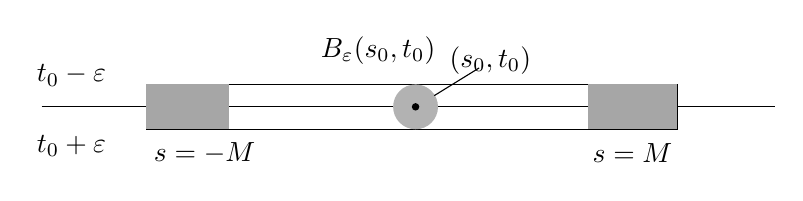
\begin{tikzpicture}[scale=0.95]
\draw (-1.4,0) -- (8.4,0);
\draw (0,-0.3) rectangle (7.1,0.3);
\fill[gray!70] (0,-0.3) rectangle (1.1,0.3);
\fill[gray!70] (5.9,-0.3) rectangle (7.1,0.3);
\fill[gray!60] (3.6,0) circle (0.3);
\fill (3.6,0) circle (0.05);
\node at (-1.0,0.42) {$t_0-\varepsilon$};
\node at (-1.0,-0.52) {$t_0+\varepsilon$};
\node at (0.78,-0.62) {$s=-M$};
\node at (6.5,-0.62) {$s=M$};
\node at (3.1,0.75) {$B_\varepsilon(s_0,t_0)$};
\node at (4.6,0.62) {$(s_0,t_0)$};
\draw (4.45,0.52) -- (3.85,0.15);
\end{tikzpicture}
\caption{}
\label{fig:strip-balls}
\end{figure}

由于这两条性质，我们尤其有
\[
\forall(s,t)\in B_\varepsilon(s_0,t_0)\text{，}\qquad
\frac{\partial v}{\partial s}(s,t)\neq 0
\ \text{与}\
v(s,t)\neq x^\pm(t)\text{。}
\]
换句话说，$B_\varepsilon(s_0,t_0)$ 的每一点都有一个\trMultiplePoint\footnote{译注：原书此处印作 “$v$ is locally constant and $(s_0,t_0)\in C(v)$”（换言之，$v$ 局部常值且 $(s_0,t_0)\in C(v)$）；疑应为“每一点都有\trMultiplePoint”之类的表述——上式刚证 $\partial v/\partial s$ 在 $B_\varepsilon(s_0,t_0)$ 上处处非零，下文性质 (3) 的括注亦明言 $(s_0,t_0)$ is not in $C(v)$，均与印文直接相抵；此处径改。——译者注}。

\begin{enumerate}[label=(\arabic*)]\setcounter{enumi}{2}
\item 由于 $[-M,M]\times[0,1]$ 是\trCompact{}的，而 $C(v)$ 是离散的，二者的交是有限的。在必要时把点 $(s_0,t_0)$ 稍微挪动一下，我们将假定：对这个有限集中的所有 $(s,t)$ 都有 $v(s_0,t_0)\neq v(s,t)$（这是可能的，因为 $v$ 在 $(s_0,t_0)$ 的一个邻域内不是常值的，因为 $(s_0,t_0)$ 不属于 $C(v)$）；并且，在缩小 $\varepsilon$ 之后，还将有
\[
v(B_\varepsilon(s_0,t_0))\cap v\bigl([-M,M]\times[0,1]\cap C(v)\bigr)=\varnothing\text{。}
\]
\end{enumerate}

\begin{figure}[htbp]
\centering
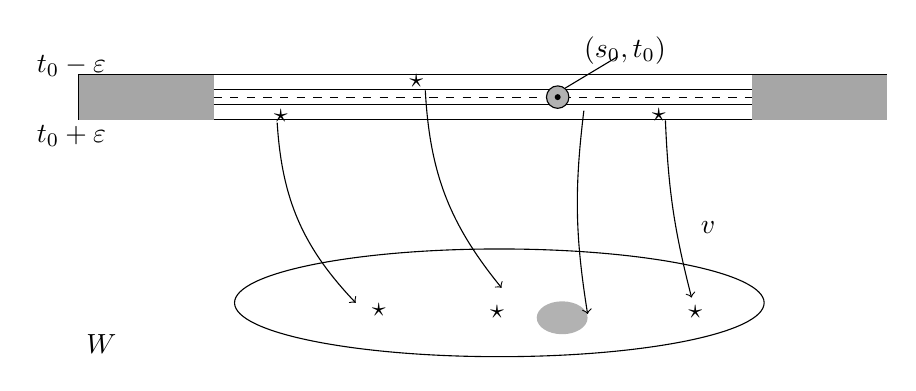
\begin{tikzpicture}[scale=0.95]
\draw (-1.8,-0.3) rectangle (9.0,0.3);
\fill[gray!70] (-1.8,-0.3) rectangle (0,0.3);
\fill[gray!70] (7.2,-0.3) rectangle (9.0,0.3);
\draw (0,0.1) -- (7.2,0.1);
\draw (0,-0.1) -- (7.2,-0.1);
\draw[dashed] (0,0) -- (7.2,0);
\fill[gray!60] (4.6,0) circle (0.15);
\draw (4.6,0) circle (0.15);
\fill (4.6,0) circle (0.04);
\node at (5.5,0.62) {$(s_0,t_0)$};
\draw (5.4,0.54) -- (4.7,0.12);
\node at (2.71,0.22) {$\star$};
\node at (0.9,-0.25) {$\star$};
\node at (5.95,-0.24) {$\star$};
\draw (3.82,-2.75) ellipse (3.54 and 0.72);
\node at (-1.5,-3.3) {$W$};
\node at (2.21,-2.85) {$\star$};
\node at (3.79,-2.87) {$\star$};
\node at (6.44,-2.87) {$\star$};
\fill[gray!60] (4.66,-2.95) ellipse (0.34 and 0.22);
\draw[->] (0.85,-0.34) to[bend right=20] (1.9,-2.75);
\draw[->] (2.83,0.09) to[bend right=18] (3.85,-2.55);
\draw[->] (4.95,-0.18) to[bend right=8] (5.0,-2.9);
\draw[->] (6.04,-0.31) to[bend right=6] (6.39,-2.68);
\node at (6.61,-1.74) {$v$};
\node at (-1.9,0.42) {$t_0-\varepsilon$};
\node at (-1.9,-0.52) {$t_0+\varepsilon$};
\end{tikzpicture}
\caption{}
\label{fig:critical-stars}
\end{figure}

\cref{fig:critical-stars} 画出了这一示意，其中的星号是 $C(v)$ 的诸点及其像。于是我们不再考虑\trMultiplePoint{}同时又是\trCriticalPoint{}的情形。从现在起只有\trInjective{}性要紧，并且对每个 $(s,t)\in B_\varepsilon(s_0,t_0)$，都存在一个 $s'\in\RR$ 使得 $s'\neq s$，且\footnote{译注：原书此式印作 “$u(s,t)=u(s',t)$ with $\frac{\partial u}{\partial s}(s',t)\neq 0$ and $|s'|\le M$, $|s'|>\varepsilon$”。其一，自\cref{thm:floer-via-cauchy-riemann}之后本段通篇讨论 $v$，两处 $u$ 显系笔误，径改；其二，由性质 (2) 只能得 $s'\notin[s_0-\varepsilon,s_0+\varepsilon]$（下文由之亦仅推出 $|\sigma_n'-s_0|\ge\varepsilon$），故 $|s'|>\varepsilon$ 疑为 $|s'-s_0|>\varepsilon$ 之脱漏，径改。——译者注}
\[
v(s,t)=v(s',t)
\qquad\text{其中 }\frac{\partial v}{\partial s}(s',t)\neq 0\
\text{且}\ |s'|\le M,\ |s'-s_0|>\varepsilon\text{。}
\]

对每个 $(s,t)$，与它有相同\trImage{}的点 $(s',t)$ 所成之集是有限的：否则这个集就会有一个极限点，而这就会蕴含 $\partial v/\partial s=0$。设 $s_1,\dots,s_N\in[-M,M]$ 是满足
\[
v(s_0,t_0)=v(s_1,t_0)=\dots=v(s_N,t_0)
\]
的那些点。

\begin{lemma}\label{thm:multiple-nearby}
对每个 $r>0$，存在一个 $\delta>0$，使得若 $|t-t_0|<\delta$ 且 $|s-s_0|<\delta$，则存在一个 $s'\in B_r(s_j)$ 使 $v(s,t)=v(s',t)$。
\end{lemma}

\begin{proof}
若情形并非如此，则存在一列趋于 $(s_0,t_0)$ 的序列 $(\sigma_n,t_n)$，使得 $(\sigma_n,t_n)$ 的\trMultiplePoint{} $(\sigma,t_n)$ 满足 $\sigma\notin B_r(s_j)$，$j=1,\dots,N$。\footnote{译注：原书此处印作 “$j=1,\dots,n$”；按上文取定的 $s_1,\dots,s_N$（$N$ 为满足 $v(s,t_0)=v(s_0,t_0)$ 的那些 $s$ 的个数），此处应为 $N$；此处径改。——译者注}设 $(\sigma_n',t_n)$ 是 $(\sigma_n,t_n)$ 的一个\trMultiplePoint。由上面的性质 (1) 我们知道 $|\sigma_n'|\le M$，由性质 (2) 知道 $|\sigma_n'-s_0|\ge\varepsilon$。

序列 $\sigma_n'$ 有一个极限点 $\sigma'$，它异于 $s_0,\dots,s_N$。此外，$v(\sigma_n',t_n)=v(\sigma_n,t_n)$，于是 $v(\sigma',t_0)=v(s_0,t_0)$，这就给出了一个矛盾。

\cref{fig:multiple-boxes} 画出了这一情形，其中 $B_\delta$ 的\trMultiplePoint{}位于浅阴影区域之中。
\end{proof}

\begin{figure}[htbp]
\centering
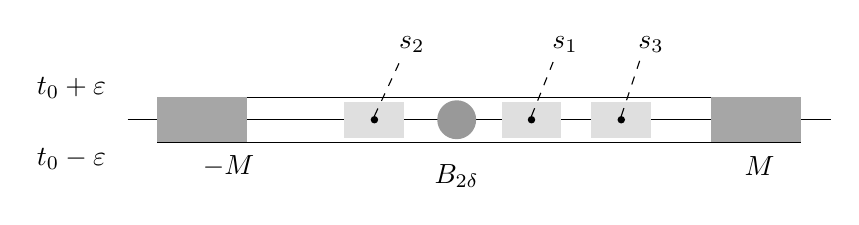
\begin{tikzpicture}[scale=0.95]
\draw (0,-0.3) rectangle (8.6,0.3);
\draw (-0.4,0) -- (9.0,0);
\fill[gray!70] (0,-0.3) rectangle (1.2,0.3);
\fill[gray!70] (7.4,-0.3) rectangle (8.6,0.3);
\node at (0.95,-0.62) {$-M$};
\node at (8.05,-0.62) {$M$};
\fill[gray!25] (2.5,-0.24) rectangle (3.3,0.24);
\fill (2.9,0) circle (0.05);
\draw[dashed] (2.9,0.05) -- (3.25,0.8);
\node at (3.4,1.0) {$s_2$};
\fill[gray!25] (4.6,-0.24) rectangle (5.4,0.24);
\fill (5.0,0) circle (0.05);
\draw[dashed] (5.0,0.05) -- (5.3,0.8);
\node at (5.45,1.0) {$s_1$};
\fill[gray!25] (5.8,-0.24) rectangle (6.6,0.24);
\fill (6.2,0) circle (0.05);
\draw[dashed] (6.2,0.05) -- (6.45,0.8);
\node at (6.6,1.0) {$s_3$};
\fill[gray!80] (4.0,0) circle (0.26);
\node at (4.0,-0.75) {$B_{2\delta}$};
\node at (-1.15,0.42) {$t_0+\varepsilon$};
\node at (-1.15,-0.52) {$t_0-\varepsilon$};
\end{tikzpicture}
\caption{}
\label{fig:multiple-boxes}
\end{figure}

既然引理到手，我们就取定一个 $r<\varepsilon/2$ 与一个相应的 $\delta$。对 $j=1,\dots,N$，我们令
\[
\Sigma_j=\bigl\{(s,t)\in\overline{B}_\delta(s_0,t_0)\ \bigm|\ v(s,t)\in v(\overline{B}_r(s_j)\times\{t\})\bigr\}\text{。}
\]
诸 $\Sigma_j$ 都是闭的，并且由上一个引理，
\[
\Sigma_1\cup\dots\cup\Sigma_N=\overline{B}_\delta(s_0,t_0)\text{，}
\]
于是其中至少有一个具有非空内部。我们假定它是 $\Sigma_1$。对于 $\Sigma_1$ 内部的一点 $(s_\star,t_\star)$ 与一个充分小的实数 $\rho>0$，我们有
\[
B_\rho(s_\star,t_\star)\subset\Sigma_1\subset B_\delta(s_0,t_0)\subset B_\varepsilon(s_0,t_0)\text{。}
\]
从而我们可以把 $r>0$ 选得充分小，使得
\[
B_r(s_i)\cap B_\varepsilon(s_0)=\varnothing
\qquad\text{对每个 }i=1,\dots,N\text{，}
\]
特别地\footnote{译注：原书上式第二个因子印作 $B_{r_1}(s_1)$；$r_1$ 全节未尝定义，按 $\Sigma_1$ 的定义（$s'\in\overline{B}_r(s_j)$）应为 $\overline{B}_r(s_1)$；此处径改。——译者注}，
\[
B_\rho(s_\star,t_\star)\cap\bigl(\overline{B}_r(s_1)\times B_\delta(t_0)\bigr)=\varnothing\text{。}
\]
\cref{fig:delta-balls} 画出了这一情形，其中 $B_\rho(s_\star,t_\star)$ 的每一点都在浅阴影区域中有一个\trMultiplePoint。

\begin{figure}[htbp]
\centering
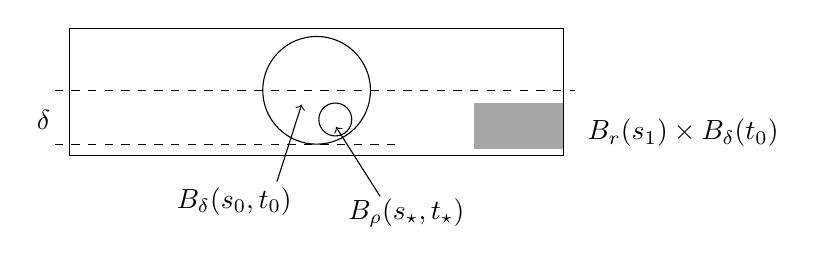
\begin{tikzpicture}[scale=0.95]
\draw (0,-0.8) rectangle (6.6,0.9);
\draw[dashed] (-0.2,0.07) -- (6.75,0.07);
\draw[dashed] (-0.2,-0.65) -- (4.43,-0.65);
\node at (-0.35,-0.33) {$\delta$};
\fill[gray!70] (5.4,-0.72) rectangle (6.6,-0.1);
\node at (8.2,-0.5) {$B_r(s_1)\times B_\delta(t_0)$};
\draw (3.3,0.07) circle (0.72);
\draw (3.55,-0.32) circle (0.22);
\node at (2.2,-1.42) {$B_\delta(s_0,t_0)$};
\draw[->] (2.77,-1.15) -- (3.1,-0.12);
\node at (4.5,-1.57) {$B_\rho(s_\star,t_\star)$};
\draw[->] (4.15,-1.35) -- (3.56,-0.42);
\end{tikzpicture}
\caption{}
\label{fig:delta-balls}
\end{figure}

按 $\Sigma_1$ 的定义，对每个 $(s,t)\in B_\rho(s_\star,t_\star)$，都存在一个 $s'\in\overline{B}_r(s_1)$ 使 $v(s,t)=v(s',t)$。特别地，存在一个 $s_\star'\neq s_\star$ 使
\[
v(s_\star,t_\star)=v(s_\star',t_\star)\text{。}
\]

我们在 $B_\varepsilon(0,0)$ 上定义两个函数 $v_1$ 与 $v_2$ 如下：
\[
\begin{array}{l}
v_1(s,t)=v(s+s_\star,t+t_\star)\\
v_2(s,t)=v(s+s_\star',t+t_\star)\text{。}
\end{array}
\]
这两个函数满足同一个\trCauchyRiemann{}方程，并且在原点处重合。此外，它们在原点处的\trDifferential{}都非零。的确，$(s_\star,t_\star)\in B_\varepsilon(s_0,t_0)$ 不属于 $C(v)$，而 $(s_\star',t_\star)$ 是 $(s_\star,t_\star)$ 的一个\trMultiplePoint，因而由性质 (3)，它也不属于 $C(v)$。于是，按构造，对每个 $(s,t)\in B_\rho(0,0)$，都存在一个 $s'\in\overline{B}_{2r}(0)$ 使 $v_1(s,t)=v_2(s',t)$。我们对这些函数应用下面的引理。它是\trContinuationPrinciple{}的一个推论（我们稍后证明）。

\begin{lemma}\label{thm:coincidence-two-solutions}
设 $v_1$ 与 $v_2$ 是 $B_\varepsilon(0)$ 上\trCauchyRiemann{}方程（于此 $X_t\equiv0$）的两个解，在 $0$ 处取相同的值，且 $(dv_1)_0$ 与 $(dv_2)_0$ 非零。再设对每个 $\varepsilon>0$，都存在一个 $\delta>0$ 使得
\[
\forall(s,t)\in B_\delta(0),\ \exists s'\in\RR
\ \text{使得 }(s',t)\in B_\varepsilon(0)
\ \text{且}\ v_1(s,t)=v_2(s',t)\text{。}
\]
则对每个 $z\in B_\varepsilon(0)$ 都有 $v_1(s,t)=v_2(s,t)$。
\end{lemma}

于是 $v_1(s,t)=v_2(s,t)$，也就是说，在 $0$ 的一个邻域内 $v(s+s_\star,t+t_\star)=v(s+s_\star',t+t_\star)$。但我们要证的是 $v_1=v_2$ 在整个 $\RR^2$ 上成立。映射 $v_1$ 与 $v_2$ 都满足\trCauchyRiemann{}方程
\[
\frac{\partial w}{\partial s}+J\frac{\partial w}{\partial t}=0\text{。}
\]
我们定义算子
\[
\begin{array}{c}
\scr{F}\colon\cC^\infty(\RR\times S^1;\RR^{2n})\longrightarrow\cC^\infty(\RR\times S^1;\RR^{2n})\\[2pt]
w\longmapsto\dfrac{\partial w}{\partial s}+J(w)\dfrac{\partial w}{\partial t}\text{。}
\end{array}
\]
于是 $\scr{F}(v_1)=\scr{F}(v_2)$。我们可以把它写成
\[
\begin{aligned}
0&=\scr{F}(v_1)-\scr{F}(v_2)\\
&=\int_0^1\frac{d}{d\tau}\scr{F}\bigl(v_1+\tau(v_2-v_1)\bigr)d\tau\\
&=\int_0^1(d\scr{F})_{v_1+\tau(v_2-v_1)}(v_2-v_1)d\tau\text{。}
\end{aligned}
\]
与\cref{sec:linearization-floer}中\trFloer{}算子的\trLinearization{}计算相类似的一个计算给出（此时 $H=0$ 而 $J$ 依赖于 $t$）
\[
(d\scr{F})_{v_1+\tau(v_2-v_1)}(Y)
=\frac{\partial Y}{\partial s}+J_0\frac{\partial Y}{\partial t}+\widetilde{S}(\tau,s,t)Y\text{，}
\]
其中 $\widetilde{S}$ 是一个映射
\[
\widetilde{S}\colon[0,1]\times\RR^2\longrightarrow\operatorname{End}(\RR^{2n})\text{。}
\]
令 $Y=v_2-v_1$，并令 $S(s,t)=\int_0^1\widetilde{S}(\tau,s,t)d\tau$。\footnote{译注：原书上式把 $(d\scr{F})_{v_1+\tau(v_2-v_1)}(Y)$ 的一阶项统一写作 $\frac{\partial Y}{\partial s}+J_0\frac{\partial Y}{\partial t}$；然而按\trLinearization{}的计算，这一阶项本是 $\frac{\partial Y}{\partial s}+J(t,w)\frac{\partial Y}{\partial t}$（$w=v_1+\tau(v_2-v_1)$），随基点 $w$ 即随 $\tau$ 而变——把 $J(t,w)$ 统一成 $J_0$ 须同步对 $Y$ 作\trFrame{}变换，不能保留同一个 $Y$ 而只对零阶项 $\widetilde{S}$ 求平均。论证可以修补：先在局部共同坐标下写出差分方程 $\frac{\partial Y}{\partial s}+J(t,v_2)\frac{\partial Y}{\partial t}+\bigl[J(t,v_2)-J(t,v_1)\bigr]\frac{\partial v_1}{\partial t}=0$，其末项随 $Y$ 一阶消失、可中值化为 $B(s,t)Y$ 型的一阶项，再就 $J(t,v_2)$ 取定\trTrivialization{}——结论可以成立，但原书现有论证省去了这一必要变换，此处照原书排印，存疑备案。——译者注}我们发现 $v_2-v_1$ 是
\[
\frac{\partial Y}{\partial s}+J_0\frac{\partial Y}{\partial t}+S\cdot Y=0
\]
的一个解，而由上所述，它在原点的一个邻域内为零。应用\trContinuationPrinciple（\cref{thm:continuation-principle}），就有 $v_1=v_2$，也就是说
\[
v(s+s_\star,t+t_\star)=v(s+s_\star',t+t_\star)
\qquad\text{对每个 }(s,t)\in\RR^2\text{。}
\]
由归纳法，对每个 $k\in\ZZ$ 都有 $v(s,t)=v(s+k(s_\star'-s_\star),t)$，\footnote{译注：原书右端印作 $v(k(s_\star'-s_\star),t)$，疑脱平移量 $s$——照印文取 $k=0$ 即得无据的 $v(s,t)=v(0,t)$，此处径改；取 $k\to\pm\infty$ 仍得 $v(s,t)=x^{\pm}(t)$，结论不变。——译者注}而取极限即得 $v(s,t)=x^\pm(t)$，这与我们所做的假设相矛盾。
\end{proof}

\subsection{\trContinuationPrinciple}
\label{subsec:continuation-principle}

现在我们必须证明\trContinuationPrinciple。我们将考虑“受\trPerturbation{}的\trCauchyRiemann{}方程”
\[
\frac{\partial Y}{\partial s}+J_0\frac{\partial Y}{\partial t}+S\cdot Y=0
\]
的情形，其中 $J_0$ 是 $\RR^{2n}$ 上的标准\trComplexStructure，而
\[
S\colon\RR^2\longrightarrow\operatorname{End}(\RR^{2n})
\]
是一个 $\cC^\infty$ 类的映射。下面就是我们一路引向的那个命题。

\begin{proposition}[\trContinuationPrinciple]\label{thm:continuation-principle}
设 $Y$ 是 $\RR^2$ 的一个\trOpen{}子集 $U$ 上受\trPerturbation{}的\trCauchyRiemann{}方程的一个解。则集合
\[
C=\bigl\{(s,t)\in U \ \bigm|\ \text{$Y$ 在 $(s,t)$ 处有一个\textbf{\trInfiniteOrderZero}（infinite-order zero）}\bigr\}
\]
在 $U$ 中既开且闭。特别地，若 $U$ 是\trConnected{}的，而且 $Y$ 在 $U$ 的一个非空\trOpen{}子集上为零，则 $Y$ 在 $U$ 上恒为零。
\end{proposition}

\begin{remark}\label{thm:infinite-order-zero}
\begin{enumerate}[label=(\arabic*)]
\item 回忆：称一个函数 $f$ 在一点 $z_0$ 处有一个\trInfiniteOrderZero，如果对每个 $k\ge 0$，
\[
\lim_{r\to0}\frac{\sup_{|z-z_0|\le r}|f(z)|}{r^k}=0\text{。}
\]
对一个 $\cC^\infty$ 类的函数 $f$ 而言，这等价于 $f$ 的各阶导数在 $z_0$ 处全部为零。
\item 一个 $\cC^\infty$ 类的函数取无穷阶零值的那些点所成之集是闭的。在\trHolomorphic{}函数（也就是说满足\trCauchyRiemann{}方程的函数）的情形，这个闭集还是开的：这就是我们所称的“解析延拓原理”。
\end{enumerate}
\end{remark}

我们将这样来证明这个命题：把它表述成 \emph{Carleman\trSimilarityPrinciple} 的一个版本的推论。我们记 $\RR^{2n}=\CC^n$。

\begin{lemma}[\trSimilarityPrinciple]\label{thm:similarity-principle}
设 $Y\colon B_\varepsilon\to\CC^n$ 是受\trPerturbation{}的\trCauchyRiemann{}方程
\[
\frac{\partial Y}{\partial s}+J_0\frac{\partial Y}{\partial t}+S\cdot Y=0
\]
的一个 $\cC^\infty$ 类解，并设 $p>2$。则存在一个数 $\delta>0$（$\delta<\varepsilon$）、一个映射 $A\in W^{1,p}(B_\delta;\mathrm{GL}(\RR^{2n}))$ 以及一个\trHolomorphic{}映射 $\sigma\colon B_\delta\to\CC^n$，使得
\[
\forall(s,t)\in B_\delta,\quad
Y(s,t)=A(s,t)\sigma(s+it)
\ \text{且}\
J_0A(s,t)=A(s,t)J_0\text{。}
\]
\end{lemma}

\begin{remark}\label{thm:similarity-principle-integrable}
更一般地，在这个陈述中我们可以假定 $Y\in W^{1,p}(B_\varepsilon;\CC^n)$ 与 $S\in L^p\bigl(B_\varepsilon;\operatorname{End}_\RR(\RR^{2n})\bigr)$，其中 $p>2$。
\end{remark}

为了证明这个\trSimilarityPrinciple，我们要用到一个事实：标准的 $\bar{\partial}$ 是一个\trFredholmOperator（这将是\cref{thm:dbar-fredholm}）。

现在让我们把用到这一原理的那些陈述（\cref{thm:dv-isolated-zeros} 与 \cref{thm:continuation-principle}）的证明写下来。

\begin{proof}[\cref{thm:continuation-principle}的证明]
清楚得很，集合 $C$ 是闭的。我们现在来证明它也是开的。设 $z_0=s_0+it_0\in C$。\cref{thm:similarity-principle} 保证存在一个邻域 $B_\delta(z_0)$，在其上
\[
Y(z)=A(z)\sigma(z)\text{，}
\]
其中 $\sigma\colon B_\delta(z_0)\to\CC^n$ 是\trHolomorphic{}的，而 $A$ 取值于 $\CC^n$ 的实\trEndomorphism{}之中。

在 $B_\delta(z_0)$ 上，$Y$ 有一个\trInfiniteOrderZero{}当且仅当 $\sigma$ 也有一个。但 $\sigma$ 在 $z_0$ 处确实有一个\trInfiniteOrderZero。的确，对 $r<\delta$，我们有
\[
\sup_{|z-z_0|\le r}|\sigma(z)|
=\sup_{|z-z_0|\le r}\bigl|A^{-1}(z)\cdot Y(z)\bigr|
\le K\sup_{|z-z_0|\le r}|Y(z)|
\]
因为 $A^{-1}$ 是连续的（因为 $A\in W^{1,p}\bigl(B_\delta;\mathrm{GL}(\RR^{2n})\bigr)$ 是连续的）。从而
\[
\lim_{r\to0}\frac{\sup_{|z-z_0|\le r}|\sigma(z)|}{r^k}=0
\qquad\text{对每个 }k\text{。}
\]
但 $\sigma$ 是一个解析函数，因此它在 $B_\delta(z_0)$ 上为零；于是 $B_\delta(z_0)\subset C$。
\end{proof}

\begin{proof}[\cref{thm:dv-isolated-zeros}的证明]
显然，若 $(dv)_0\neq 0$，则所述为真。设 $(dv)_0=0$。映射 $v$ 是方程
\[
\frac{\partial v}{\partial s}+J\frac{\partial v}{\partial t}=0
\]
的一个解。于是，正如我们已经指出过的（\cref{thm:df-kernel-nontrivial}），$\partial v/\partial s$ 是\trLinearization{}的\trCauchyRiemann{}方程的一个解。从而我们可以把\trSimilarityPrinciple（\cref{thm:similarity-principle}）应用于 $Y=\partial v/\partial s$，得到
\[
Y(s,t)=A(s,t)\sigma(s,t)
\]
其中 $\sigma$ 在 $0$ 的一个邻域内是\trHolomorphic{}的。引理随之得证：$\sigma$ 的诸零点是\trIsolated{}的，因而 $Y=\partial v/\partial s$ 的零点亦然，$dv$ 的零点就更不必说了。
\end{proof}

从\trContinuationPrinciple{}出发，我们现在推出\cref{thm:coincidence-two-solutions}的一个证明。

\begin{proof}[\cref{thm:coincidence-two-solutions}的证明]
我们选一个 $\varepsilon>0$，它充分小，使得 $v_2\colon B_\varepsilon\to\RR^{2n}$ 把 $B_\varepsilon$ 嵌成一个\trSubmanifold{} $\Sigma=v_2(B_\varepsilon)\subset\RR^{2n}$；\footnote{译注：原书此处印作 $\Sigma=v(B_\varepsilon)$；本证明自首句起通篇讨论 $v_2$，应为 $v_2(B_\varepsilon)$；此处径改。——译者注}这样做之所以许可，是由于 $(dv_2)_0\neq 0$ 这一事实。利用一个从这个\trSubmanifold{}的一个邻域 $U_\varepsilon$ 到这个\trSubmanifold{}上的投射，我们推出一个 $\cC^\infty$ 类的映射 $\varphi$：
\[
\varphi\colon U_\varepsilon\longrightarrow B_\varepsilon
\qquad\text{且}\ \varphi|_\Sigma=v_2^{-1}\text{。}
\]
对充分小的 $\delta$，$v_1(B_\delta)\subset\Sigma$（按假设），于是我们有一个映射
\[
\varphi\circ v_1\colon B_\delta\longrightarrow U_\varepsilon\longrightarrow B_\varepsilon
\]
它按我们的假设必形如
\[
\varphi\circ v_1(s,t)=(f(s,t),t)
\]
其中 $f$ 是 $\cC^\infty$ 类的，定义在 $B_\delta(0)$ 上而取值于 $B_\varepsilon(0)$ 中。于是对 $(s,t)\in B_\delta$，我们有 $v_1(s,t)=v_2(f(s,t),t)$。由于 $v_1$ 是一个解，我们还有
\[
\begin{aligned}
0&=\frac{\partial v_1}{\partial s}(s,t)+J(t,v_1)\frac{\partial v_1}{\partial t}(s,t)
=\frac{\partial v_2}{\partial s}\bigl(f(s,t),t\bigr)\frac{\partial f}{\partial s}\\
&\qquad+J\bigl(t,v_2(f(s,t),t)\bigr)\Bigl[\frac{\partial v_2}{\partial s}\bigl(f(s,t),t\bigr)\frac{\partial f}{\partial t}
+\frac{\partial v_2}{\partial t}\bigl(f(s,t),t\bigr)\Bigr]\text{。}
\end{aligned}
\]
其次，我们利用 $v_2$ 也是一个解这一事实，也就是说
\[
J\frac{\partial v_2}{\partial t}=-\frac{\partial v_2}{\partial s}
\qquad\text{与}\qquad
J\frac{\partial v_2}{\partial s}=\frac{\partial v_2}{\partial t}\text{，}
\]
来得到
\[
\frac{\partial v_2}{\partial s}(f,t)\Bigl(\frac{\partial f}{\partial s}-1\Bigr)
+\frac{\partial v_2}{\partial t}(f,t)\frac{\partial f}{\partial t}=0\text{，}
\]
这是介于两个无关的向量 $\bigl(\partial v_2/\partial s\bigr)(f,t)$ 与 $\bigl(\partial v_2/\partial t\bigr)(f,t)$ 之间的一个线性关系。从而
\[
\frac{\partial f}{\partial s}=1
\qquad\text{与}\qquad
\frac{\partial f}{\partial t}=0\text{，}
\]
于是 $f$ 形如 $f(s,t)=s+s_0$，其中某个 $s_0\in\left]-\varepsilon,\varepsilon\right[$，而且这个 $s_0$ 还必须为零，因为 $v_2(s_0,0)=v_1(0)=v_2(0)$ 而 $v_2$ 在 $B_\varepsilon(0)$ 上是\trInjective{}的。由此得到 $f(s,t)=s$，这意味着 $v_1$ 与 $v_2$ 在定义 $f$ 的 $0$ 的那个邻域内重合。由\trContinuationPrinciple，$v_1$ 与 $v_2$ 必在整个 $B_\varepsilon$ 上重合。
\end{proof}

\begin{proof}[\cref{thm:similarity-principle}的证明]
尚需满足的最后一个条件是：$A(s,t)$ 对一切 $(s,t)$ 都是一个 $\CC$-线性映射（也就是说与用 $i$ 作乘法交换，我们曾把这个乘法记作 $J_0$）。

让我们尝试把（受\trPerturbation{}的\trCauchyRiemann{}方程中的）$S$ 换成一个 $\CC$-线性映射。我们先写
\[
S^+=\frac{1}{2}(S-J_0SJ_0)
\qquad\text{与}\qquad
S^-=\frac{1}{2}(S+J_0SJ_0)\text{，}
\]
于是 $S=S^++S^-$，并且
\[
J_0S^+=\frac{1}{2}(J_0S+SJ_0)=S^+J_0\text{；}
\]
因而 $S^+$ 是 $\CC$-线性的，而 $S^-$ 是反 $\CC$-线性的。对 $(s,t)\in B_\varepsilon$，我们如下定义 $D(s,t)\in\operatorname{End}_\RR(\CC^n)$：
\[
D(s,t)\cdot Z=
\begin{cases}
\dfrac{1}{\|Y(s,t)\|^2}\cdot\bigl(Y(s,t)\cdot{}^tY(s,t)\bigr)\cdot\overline{Z}
&\text{若 } Y(s,t)\neq 0\text{，}\\[8pt]
0
&\text{若 } Y(s,t)=0\text{。}
\end{cases}
\]
注意到当 $Y(s,t)\neq 0$ 时，我们有
\[
D(s,t)\cdot Z=\frac{\langle Y,Z\rangle}{\|Y\|^2}(s,t)\cdot Y(s,t)\text{，}
\]
其中 $\langle\cdot,\cdot\rangle$ 表示 $\CC^n$ 上通常的\trHermitian{}\trInnerProduct（\cref{sec:complex-structures}）。特别地，对一切 $(s,t)$ 都有 $DY=Y$。此外，这个映射显然是反 $\CC$-线性的。最后我们看到
\[
\|D(s,t)\|\le 1
\qquad\text{对一切 }(s,t)\text{，}
\]
这尤其蕴含
\[
S^-\cdot D\in L^p\bigl(B_\varepsilon,\operatorname{End}_\RR(\RR^{2n})\bigr)\text{。}
\]
其次，我们令
\[
\widetilde{S}(s,t)=S^+(s,t)+S^-(s,t)\cdot D(s,t)\text{，}
\]
从而定义了一个 $\CC$-线性映射 $\widetilde{S}$，
\[
\widetilde{S}\in L^p\bigl(B_\varepsilon,\operatorname{End}_\RR(\RR^{2n})\bigr)\text{，}
\]
它满足
\[
\widetilde{S}\cdot Y=S^+Y+S^-DY=S^+Y+S^-Y=SY\text{，}
\]
于是 $Y$ 也是把 $S$ 换成 $\widetilde{S}$ 之后的那个方程的解。从而我们可以假定方程中的 $S$ 是 $\CC$-线性的。所想要的结果是下面这个引理的一个推论。

\begin{lemma}\label{thm:fundamental-matrix}
存在一个 $\delta\in\left]0,\varepsilon\right]$ 与一个 $A\in W^{1,p}\bigl(B_\delta;\operatorname{End}(\RR^{2n})\bigr)$ 使得
\[
\frac{\partial A}{\partial s}+J_0\frac{\partial A}{\partial t}+S\cdot A=0
\]
且 $A(0,0)=\mathrm{Id}$。
\end{lemma}

在这个陈述中，乘积 $S\cdot A$ 是 $L^p\bigl(B_\delta;\operatorname{End}(\RR^{2n})\bigr)$ 的一个元素（由\cref{thm:w1p-product-inequality}）。让我们先承认这个引理（暂时！），并把\cref{thm:similarity-principle}的证明做完。设 $A$ 如引理所述，若它不是 $\CC$-线性的，就用
\[
A^+=\frac{1}{2}(A-J_0AJ_0)
\]
来代替它，后者是同一个方程的解（因为我们已假定 $S$ 是 $\CC$-线性的），而且也满足 $A^+(0,0)=\mathrm{Id}$。于是我们可以、而且也确实因此假定 $A$ 与 $J_0$ 交换。现在让我们证明它也满足\cref{thm:similarity-principle}所宣布的其余条件。由于 $A(0,0)=\mathrm{Id}$，只要把 $\delta$ 选得充分小，$A(s,t)$ 对 $(s,t)\in B_\delta$ 就是\trInvertible{}的。其次，令
\[
\sigma=A^{-1}\cdot Y\text{，}
\qquad\text{于是 }Y=A\cdot\sigma\text{。}
\]
由于 $Y$ 是方程的一个解，我们有
\[
\frac{\partial(A\sigma)}{\partial s}+J_0\frac{\partial(A\sigma)}{\partial t}+S\cdot(A\sigma)=0\text{，}
\]
亦即
\[
\frac{\partial A}{\partial s}\sigma+A\frac{\partial\sigma}{\partial s}
+J_0\frac{\partial A}{\partial t}\sigma+J_0A\frac{\partial\sigma}{\partial t}+S\cdot A\sigma=0\text{，}
\]
这蕴含
\[
A\Bigl(\frac{\partial\sigma}{\partial s}+J_0\frac{\partial\sigma}{\partial t}\Bigr)=0\text{，}
\]
从而 $\sigma$ 是\trHolomorphic{}的（它是连续的，因为它等于 $\sigma=A^{-1}\cdot Y$；而由\trEllipticRegularity，它是 $\cC^\infty$ 的）。

\begin{proof}[\cref{thm:fundamental-matrix}的证明]
我们所要找的矩阵 $A$ 是我们方程的解的一个基本矩阵。只需对“向量”$Y\in W^{1,p}(B_\delta;\RR^{2n})$ 考虑方程
\[
\frac{\partial Y}{\partial s}+J_0\frac{\partial Y}{\partial t}+S\cdot Y=0\text{，}
\]
并证明：对每个固定的 $v_0\in\RR^{2n}$，它都有一个满足 $Y(0,0)=v_0$ 的解。利用\trCanonical{}基的诸向量，我们便会得到矩阵 $A$ 的各列。

为此，考虑
\[
B_\delta\subset\CC\subset\CC\cup\{\infty\}=S^2\text{。}
\]
若 $Y$ 是从 $S^2$ 到 $\CC^n=\RR^{2n}$ 的一个映射，则 $\bar{\partial}Y$ 是\trVectorBundle{} $\bigl(\Lambda^{0,1}T^\star S^2\bigr)^n=\Lambda^{0,1}T^\star S^2\otimes\CC^n$ 的一个\trSection，而等式 $\bar{\partial}Y=0$ 就意味着 $Y$ 是 $\CC^n$ 中的一张\trHolomorphic{}\trSphere。

现在我们可以使用下面这个定理所回顾的 $\bar{\partial}$ 的本质性质（它是 \trCalderonZygmund{} 不等式的一个推论；见\cref{thm:calderon-zygmund-inequality}）。

\begin{theorem}\label{thm:dbar-fredholm}
对每个 $p>1$，算子
\[
\bar{\partial}\colon W^{1,p}(S^2,\CC^n)\longrightarrow
L^p\bigl(\Lambda^{0,1}T^\star S^2\otimes\CC^n\bigr)
\]
是一个\trSurjective{}的\trFredholmOperator。
\end{theorem}

构成\cref{thm:symplectic-area-nonzero}之证明的那个计算表明：若 $\bar{\partial}Y=0$，则
\[
\int_{\RR^2}\Bigl\|\frac{\partial Y}{\partial t}\Bigr\|^2ds\,dt=\int_{S^2}Y^\star\omega=0
\]
（应用\trStokes{}公式）。于是 $\bar{\partial}$ 的\trKernel{}只含常值映射，从而其维数为 $2n$；而且由于 $\bar{\partial}$ 是\trSurjective{}的，它的\trIndex{}也等于 $2n$。其次，考虑算子
\[
\begin{array}{c}
D\colon W^{1,p}(S^2;\CC^n)\longrightarrow L^p\bigl(\bigl(\Lambda^{0,1}T^\star S^2\bigr)^n\bigr)\oplus\CC^n\\[2pt]
Y\longmapsto(\bar{\partial}Y,Y(0))\text{。}
\end{array}
\]
它是
\[
(\bar{\partial},0)\colon W^{1,p}(S^2;\CC^n)\longrightarrow
L^p\bigl(\bigl(\Lambda^{0,1}T^\star S^2\bigr)^n\bigr)\oplus\CC^n\text{，}
\]
它是\trIndex{}为 $0$ 的\trFredholmOperator，与算子 $Y\mapsto(0,Y(0))$ 之和——后者是紧的，因为 $W^{1,p}$ 到 $L^\infty$ 有一个连续的\trEmbedding。由\cref{thm:appC-compact-perturbation-index}，我们知道它也是\trIndex{}为 $0$ 的\trFredholmOperator。但它的\trKernel{}仅由零常值组成，因而为零。从而 $D$ 是\trBijective{}的。

设 $D_\delta$ 是 $D$ 的如下定义的小\trPerturbation：
\[
D_\delta(Y)=\bigl(\bar{\partial}Y+S_\delta\cdot Y\,d\overline{Z},\,Y(0)\bigr)\text{，}
\]
其中 $S_\delta\colon\CC\cup\{\infty\}\to\operatorname{End}_\RR(\CC^n)$ 又由
\[
S_\delta(s,t)=
\begin{cases}
S(s,t) & \text{若 }(s,t)\in B_\delta\text{，}\\
0 & \text{否则}
\end{cases}
\]
定义。清楚得很，
\[
\lim_{\delta\to0}\|S_\delta\|_{L^p}=0\text{，}
\qquad\text{从而}\qquad
\lim_{\delta\to0}\|D_\delta-D\|^{\mathrm{op}}=0\text{，}
\]
因而当 $\delta$ 充分小时 $D_\delta$ 也是\trBijective{}的。取定这样一个数 $\delta$ 之后，我们取一个 $Y$ 使得 $D_\delta Y=(0,v_0)$。它在 $B_\delta$ 上的限制满足受\trPerturbation{}的\trCauchyRiemann{}方程与“初始条件”$Y(0)=v_0$，这就证明了引理（\cref{thm:fundamental-matrix}）……
\end{proof}

……以及\trSimilarityPrinciple（\cref{thm:similarity-principle}）。
\end{proof}

我们本可以采用与\trIndex{}的计算（将于\cref{sec:index-computation}中给出）相同的办法来做这件事：这正是\cref{ex:ch14-045-fredholm-another-proof}的对象。
